% Compile with XeLaTeX or LuaLaTeX
\documentclass[12pt]{article}
\usepackage[vmargin=0.5in, hmargin=1.25in]{geometry}

%%% Language support
\usepackage[english]{babel} % Get everything translated properly
%\usepackage[latin1]{inputenc} % Input text correctly
\usepackage[T1]{fontenc} % Get hyphenation right
\usepackage{lmodern} % The Latin Modern fonts

%%%Typesetting support
\usepackage{fontspec}
\usepackage{xcolor}
\usepackage[uppercase]{titlesec}
\usepackage{titling}

%%% Set fonts and section styles
\defaultfontfeatures{Ligatures=TeX}
% Set sans font to Helvetica Neue Light
\setsansfont{HelveticaNeue Light}
% Set serifed font to Garamond
\setmainfont{EB Garamond}
% Define light and dark Microsoft blue colours
\definecolor{MSBlue}{rgb}{.204,.353,.541}
\definecolor{MSLightBlue}{rgb}{.31,.506,.741}
% Set title and section formats
\newfontfamily\headingfont[]{HelveticaNeue Light}
\titleformat*{\section}{\Large\headingfont\color{MSBlue}}
\titleformat*{\subsection}{\Large\headingfont}
\titleformat*{\subsubsection}{\large\headingfont}

%\titleformat{\subsection} [block]{\large\bfseries\filcenter}{}{0em}{\MakeUppercase
%\titleformat{\subsection}[block]{\large\headingfont\filcenter}{}{0em}{\MakeUppercase}
\renewcommand{\maketitlehooka}{\headingfont\color{MSBlue}}


\title{\uppercase{Eligibility criteria for BlockchainX constituents and exchanges}}
\author{Håkan Holmberg}
\date{\today}


% https://tex.stackexchange.com/questions/48307/how-do-you-put-multiple-paragraphs-in-a-caption
\usepackage[pdftex]{graphicx}
\usepackage{hyperref}

\begin{document}

\maketitle

In order to avoid unacceptable market, counterparty and operational risks,
exchanges used to price index constituents as well as index constituents themselves need to fulfill certain eligibility
criteria. These criteria are continuously reviewed by the BlockchainX index
committee in order to stay relevant as a measure of risk reduction.

\begin{figure}
\centering
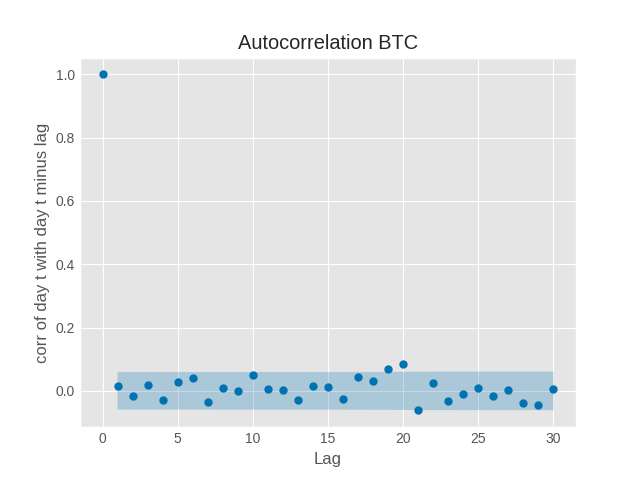
\includegraphics{output/bsk/ret/ACF_btc.png}
\caption{caption. caption. caption. caption. caption. caption. caption. caption. caption. caption. caption. caption. caption. caption. caption. caption. caption. caption. caption. caption. caption. caption. caption. caption. caption. caption. caption. caption. caption. caption. caption. caption. caption. caption. caption. caption. caption. caption. caption. caption.

caption. caption. caption. caption. caption. caption. caption. caption. caption. caption. caption. caption. caption.

caption. caption. caption. caption. caption. caption. caption. caption. caption. caption. caption. caption. caption. caption. caption. caption. caption. caption. caption. caption. caption. caption. caption. caption. caption. caption. caption. caption. caption. caption. caption. caption. caption. caption. caption.

caption. caption. caption. caption. caption. caption. caption.}
\end{figure}


\section*{Eligibility criteria for exchanges used to price index constituents}

Exchanges are used to compute the composite value of the BlockchainX
index. As such, they are integral to all aspects of both the blockhainX index
and investment products that aim to track it. Exhcanges are always used in order
to ensure that the index is priced using primary data sources in order to ensure accuracy of provided data and the
possibility to trade at source price. Furthermore, European Securities and Market
Authority (ESMA) suggests that primary data
sources are used in index construction. As of \today \  an exchange is
eligible to price index constituents if it has:

\end{document}
